\section{Design of the equalizer}
This chapter aims to describe the design of an digital equalizer, for an electric guitar. 
To begin with, some design choices have to made. From \autoref{tab:frequency_area} it is seen that the frequency area of an electric guitar is from \SI{80}{\hertz} to \SI{4400}{\hertz}. Thus the equalizer has to be able to change the frequency response in this area. This change in the frequency response is made by as series connection of shelving filters and peak filters. The shelving filters are used the highest and the lowest bands of the equalizer and the peak filters are used for the in between bands. All filters are normally kept as first or second order filters. 

The transferfunction for a first order analog low shelving filter is as in \autoref{eq:analog_shelving_low}, and the transferfunction for a first order analog high shelving filter is as in \autoref{eq:analog_shelving_high} \citep{Julius_smith}:

\begin{equation}\label{eq:analog_shelving_low}
        H(s) = 1+\frac{G\cdot\omega_1}{s+\omega_1}
    \end{equation}

    \startexplain
     \explain{$\omega_1$ is the transition frequency between the high and the low frequency regions}{\si{\radian/\second}}
     \explain{$G$ is the transition frequency between the high and the low frequency regions}{\si{\radian/\second}}
    \stopexplain

\begin{equation}\label{eq:analog_shelving_high}
        H(s) = 1+\frac{G\cdot\frac{1}{\omega_1}}{\frac{1}{s}+\frac{1}{\omega_1}}
    \end{equation}
    
In \autoref{fig:low_and_high_shelving} a bodeplot of first order low- and high- shelving filters with different transition frequencies is shown.

\begin{figure}
    \centering
        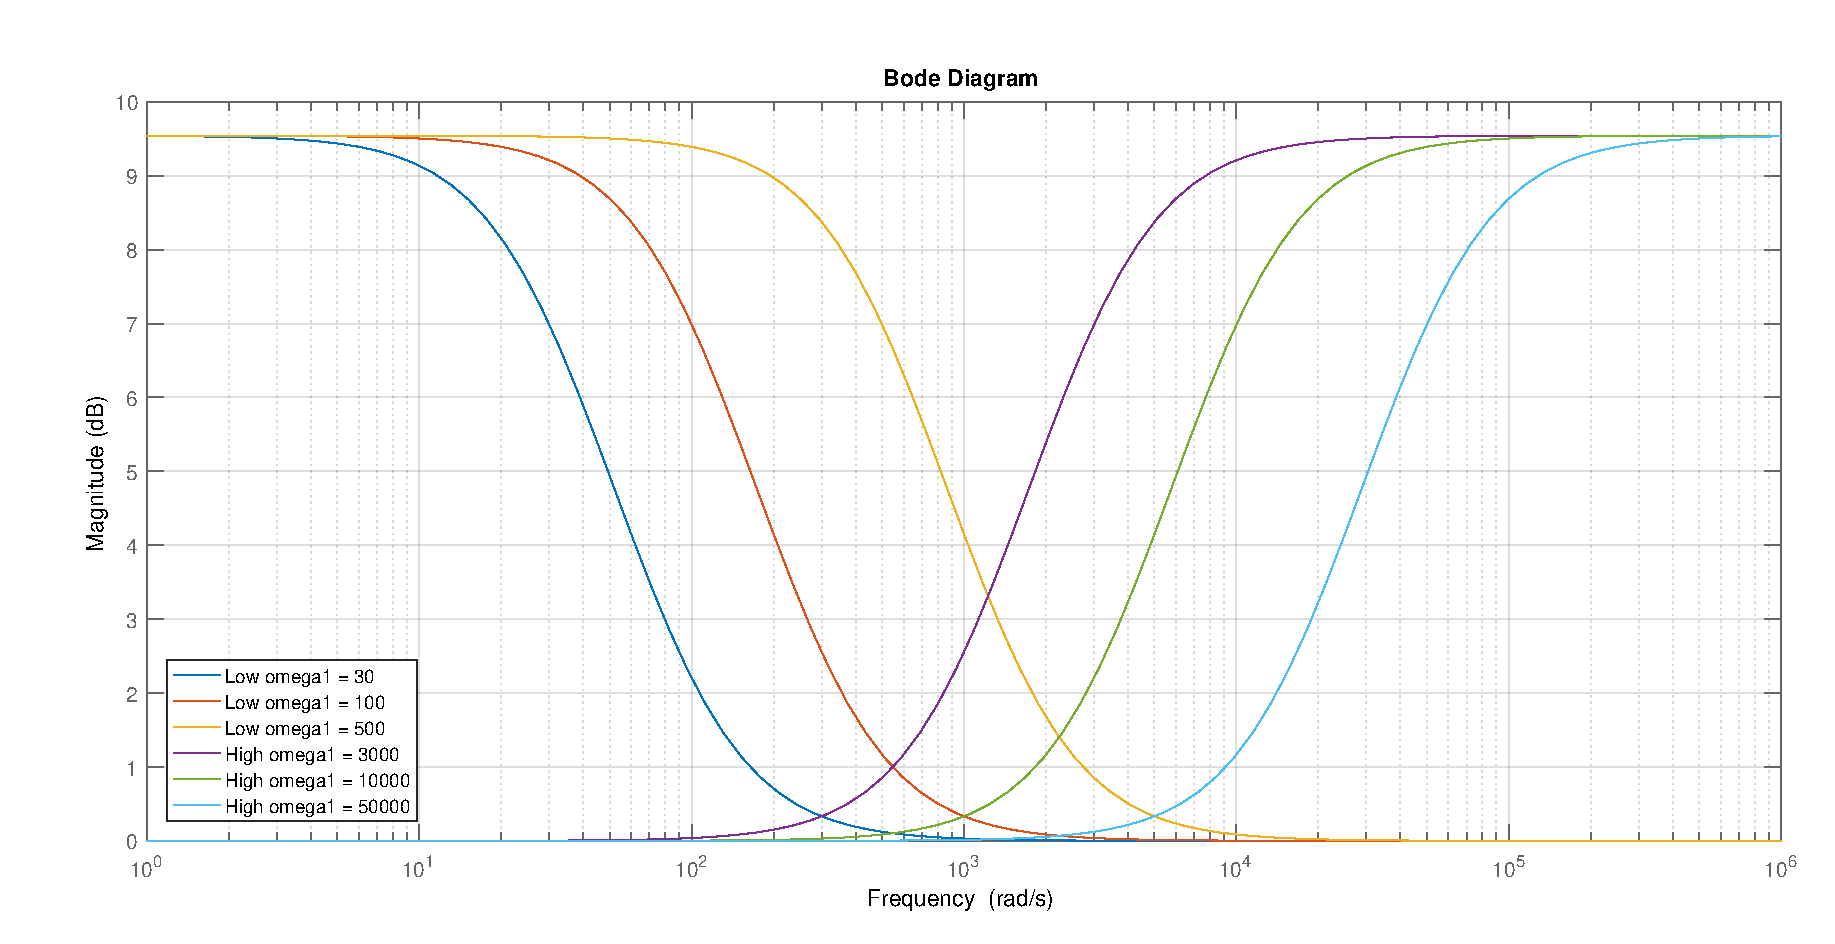
\includegraphics[width=\textwidth]{low_and_high_shelfing.pdf}
        \caption{Bodeplot of first order low- and high- shelving filters with different transition frequencies.}
        \label{fig:low_and_high_shelving}
  \end{figure} 


%Raised Cosine

%The interference effects on the side lying bandpass filter can easily be avoided by using an digital equalizer with third-octave raised cosine characteristics. The difference between the  bandpass filter characteristics and the one with a raised-cosine are shown in \autoref{fig:raised_cosine_vs_traditional}
%
%\begin{figure} [htbp]
% \centering
%  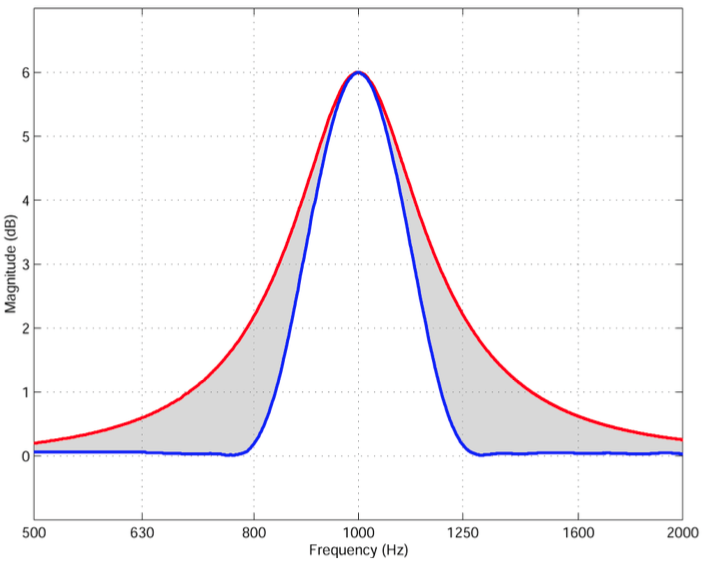
\includegraphics[width=0.7\textwidth]{raised_cosine_vs_traditional}
%  \caption{The photo shows the raised cosine bandpass filter characteristics versus traditional characteristics of third-octave bandpass filter \citep{nordic}
%  }
%  \label{fig:raised_cosine_vs_traditional}
%\end{figure}
%
%
%
%When using third-octave raised cosine bandpass filter, it is possible to make an equalizer where neighboring filters do not interfere with each other, or explained i another way, they interfere the right way, because a raised cosine filter does not leak into other third-octave bands like the traditional filter does. With this kind of filter it is possible to make a perfectly flat frequency response, and it is very close to an ideal equalizer. The \autoref{fig:raised_cosine_respond} shows the frequency response of a third-octave raised cosine equalizer designed by Dolby lake with the same gain and frequency settings as the analog equalizer at \autoref{fig:analog_equalizer}.
%
%\begin{figure} [htbp]
% \centering
%  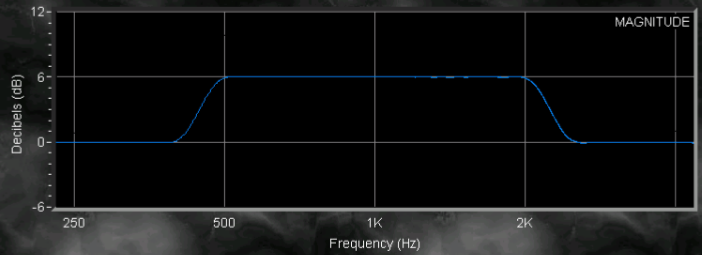
\includegraphics[width=0.8\textwidth]{raised_cosine_respond}
%  \caption{The photo shows an third-octave raised cosine equalizer frequency response  \citep{nordic}
%  }
%  \label{fig:raised_cosine_respond}
%\end{figure}
%
%
%The equalizer is used to compensate for the changes in sound due to different room characteristics, because the sound can be completely different in different rooms. The room characteristics will or can amplify or attenuate some frequency, and therefore the equalizer is very important to adjust the frequency in every new room.\citep{howtogeek} 
